\documentclass[tikz,border=8pt]{standalone}
\usepackage{tikz}
\usetikzlibrary{positioning, arrows.meta}

\begin{document}
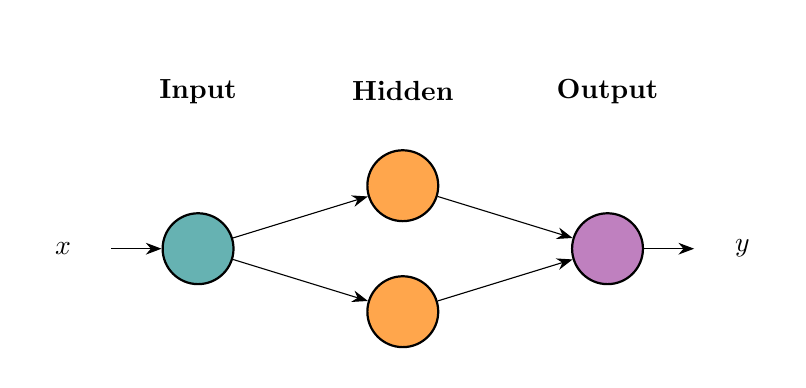
\begin{tikzpicture}[
    every node/.style = {circle, draw=black, thick, minimum size=0.9cm},
    input/.style  = {fill=teal!60},
    hidden/.style = {fill=orange!70},
    output/.style = {fill=violet!50},
    label/.style  = {draw=none, fill=none, font=\bfseries},
    wlabel/.style = {draw=none, fill=none, shape=rectangle, font=\scriptsize, inner sep=1pt},
    >={Stealth[length=2mm]}
]

% input node
\node[input] (x) at (0, -0.8) {};
\coordinate (xin) at (-1.1, -0.8);
\node[draw=none, fill=none, left=0.15cm of xin] {$x$};

% hidden layer
\node[hidden] (h1) at (2.6, 0)    {};
\node[hidden] (h2) at (2.6, -1.6) {};

% output node
\node[output] (y) at (5.2, -0.8) {};
\coordinate (yout) at (6.3, -0.8);
\node[draw=none, fill=none, right=0.15cm of yout] {$y$};

% layer labels, all at the same height
\node[label] at (0,   1.2) {Input};
\node[label] at (2.6, 1.2) {Hidden};
\node[label] at (5.2, 1.2) {Output};

% arrow in and out
\draw[->] (xin) -- (x);
\draw[->] (y) -- (yout);

% connections: input -> hidden
\draw[->] (x) -- (h1) node[wlabel, midway, above, sloped] {};
\draw[->] (x) -- (h2) node[wlabel, midway, below, sloped] {};

% connections: hidden -> output
\draw[->] (h1) -- (y) node[wlabel, midway, above, sloped] {};
\draw[->] (h2) -- (y) node[wlabel, midway, below, sloped] {};

\end{tikzpicture}
\end{document}
